% EJC papers *must* begin with the following two lines. 
\documentclass[12pt]{article}
\usepackage{e-jc}

% Please remove all other commands that change parameters such as
% margins or pagesizes.

% only use standard LaTeX packages
% only include packages that you actually need

% we recommend these ams packages
\usepackage{amsthm,amsmath,amssymb}
\usepackage{verbatim}

% we recommend the graphicx package for importing figures
\usepackage{graphicx}

% use this command to create hyperlinks (optional and recommended)
\usepackage[colorlinks=true,citecolor=black,linkcolor=black,urlcolor=blue]{hyperref}

% use these commands for typesetting doi and arXiv references in the bibliography
\newcommand{\doi}[1]{\href{http://dx.doi.org/#1}{\texttt{doi:#1}}}
\newcommand{\arxiv}[1]{\href{http://arxiv.org/abs/#1}{\texttt{arXiv:#1}}}

% all overfull boxes must be fixed; 
% i.e. there must be no text protruding into the margins


% declare theorem-like environments
\theoremstyle{plain}
\newtheorem{theorem}{Theorem}
\newtheorem{lemma}[theorem]{Lemma}
\newtheorem{corollary}[theorem]{Corollary}
\newtheorem{proposition}[theorem]{Proposition}
\newtheorem{fact}[theorem]{Fact}
\newtheorem{observation}[theorem]{Observation}
\newtheorem{claim}[theorem]{Claim}

\theoremstyle{definition}
\newtheorem{definition}[theorem]{Definition}
\newtheorem{example}[theorem]{Example}
\newtheorem{conjecture}[theorem]{Conjecture}
\newtheorem{open}[theorem]{Open Problem}
\newtheorem{problem}[theorem]{Problem}
\newtheorem{question}[theorem]{Question}

\theoremstyle{remark}
\newtheorem{remark}[theorem]{Remark}
\newtheorem{note}[theorem]{Note}
\newcommand{\F}{\mathcal{F}}
\newcommand{\A}{\mathcal{A}}
\newcommand{\B}{\mathcal{B}}

%%%%%%%%%%%%%%%%%%%%%%%%%%%%%%%%%%%%%%%%%%%%%%%%%%%%%%%

% if needed include a line break (\\) at an appropriate place in the title

\title{\bf An Extension of a Result of Das-Gan-Sudakov}

% input author, affilliation, address and support information as follows;
% the address should include the country, and does not have to include
% the street address 

\author{Erik Waingarten\\
\small Department of Mathematics\\[-0.8ex]
\small Massachusetts Institute of Technology\\[-0.8ex] 
\small Cambridge, MA\\
\small\tt eaw@mit.edu\\
\and
Fermi Ma\\
\small Department of Mathematics\\[-0.8ex]
\small Massachusetts Institute of Technology\\[-0.8ex]
\small Cambridge, MA\\
\small\tt fermima@mit.edu
}

% \date{\dateline{submission date}{acceptance date}\\
% \small Mathematics Subject Classifications: comma separated list of
% MSC codes available from http://www.ams.org/mathscinet/freeTools.html}

\date{\dateline{August, 2014}{XX}\\
\small Mathematics Subject Classifications: XX}

\begin{document}

\maketitle

% E-JC papers must include an abstract. The abstract should consist of a
% succinct statement of background followed by a listing of the
% principal new results that are to be found in the paper. The abstract
% should be informative, clear, and as complete as possible. Phrases
% like "we investigate..." or "we study..." should be kept to a minimum
% in favor of "we prove that..."  or "we show that...".  Do not
% include equation numbers, unexpanded citations (such as "[23]"), or
% any other references to things in the paper that are not defined in
% the abstract. The abstract will be distributed without the rest of the
% paper so it must be entirely self-contained.

\begin{abstract}
  A result of Shagnik Das, Wenying Gan, and Benny Sudakov shows that

  % keywords are optional
  \bigskip\noindent \textbf{Keywords:} Sperner's Theorem; Group Actions; Minimizing 2-chains\end{abstract}

\section{Introduction}

Let $B_n$ denote the poset of all subsets of $[n]$, where $F_1 \leq F_2$ if $F_1 \subseteq F_2$ as sets. A 2-chain is any pair of sets $F_1$ and $F_2$ such that $F_1 \subset F_2$. Sperner's Theorem states that any family of $B_n$ with no 2-chains has at most $\binom{n}{\lfloor n/2 \rfloor}$, a bound that can be shown to be tight by considering all the subsets of $[n]$ with size $\lfloor n/2 \rfloor$. Kleitman considered the related question of determining the minimum number of a 2-chains that must appear in a family of sets larger than $\binom{n}{\lfloor n/2 \rfloor}$. Das, Gan, and Sudakov considered this problem independently, and completely characterized all extremal families.

We analyze this problem for posets of the form $B_n / G$, where $G$ is subgroup of $S_n$.


%%%%%%%%%%%%%%%%%%%%%%%%%%%%%%%%%%%%%%%%%%%%%%%%%%%%%%%
\section{Background and Notation}

%This section needs a lot of work

$B_n$ denotes the poset of all subsets of $[n]$, ordered by set inclusion. When we consider groups $G$, we say two elements $x, y$ of a set $S$ are in the same orbit if $\pi(x) = y$ for some $\pi \in G$. Thus, the orbits given by $G$ partition $S$ into disjoint, nonempty subsets. The set of all $G$-orbits of $S$ is denoted $S / G$, and in this paper we will consider the poset $B_n / G$ [Stanley]. 

We will talk about the levels of $B_n$ and $B_n/G$. The $l$th level denotes all of the elements of $B_n$ or $B_n/G$ with cardinality $l$. 

Pick an arbritrary order within the elements of each level. Now order each level so that the middle level is the lowest, followed by the level above, and then the level below the middle, and then the level above, etc... Call $I_r$ the first $r$ elements in this ordering. 

%borrowed some wording from Stanley for the first paragraph. that needs to be fixed at some point.

We also use notation from [Das]. The $\ell$-shadow of a family is given by $\partial^{\ell}\F = \{G: \exists F \in \F, G \in F, |G| = |F| - \ell\}$.


%%%%%%%%%%%%%%%%%%%%%%%%%%%%%%%%%%%%%%%%%%%%%%%%%%%%%%%
\section{Groups Generated By a Transposition}

In this section, we restrict our attention to posets of the form $B_n / G$, where $G$ is a subgroup of the symmetric group $S_n$ on $n$ elements generated by a single transposition. WLOG, let the transposition be $(12)$, and denote by $G_{(12)}$ the two-element group generated by that transposition

Sperner's Theorem states that no antichain in $B_n$ is larger than the largest level $P_i$ [Stanley]. [Stanley] shows how to extend the theorem to $B_n / G$ for all finite groups $G$. 

The $i$th level of $B_n / G_{(12)}$ has size $\binom{n-2}{i-2} + \binom{n-1}{i}$, where the first term in the sum counts the number of sets that include both 1 and 2, while the second term counts the sets where at most one element of $\{1,2\}$ is included. Because $B_n / G$ is rank-symmetric and unimodal, the largest level has $\binom{n-2}{\lfloor n/2 \rfloor -2} + \binom{n-1}{\lfloor n/2 \rfloor}$ elements, which is also the size of the largest family containing no 2-chains [Stanley].

%must add citations

Theorem 1.2 of [Das] completely characterizes the minimum number of 2-chains in families $\F$ of subsets of $B_n$. We present a similar result for families $\F$ of subsets of $B_n / G$, where $G$ is a group generated by a transposition.

%% Still need to make the statement of this lemma a lot more clear

The following Lemma is due to [Das]. We restate it here for clarity, but an interested reader can find the full proof in [Das].

\begin{lemma}
\label{lemma2}
Let $G$ be a bipartite graph on $U \cup V$ with minimum degree $\delta_U \geq 1$ in $U$ and maximum degree $\Delta_V$ in $V$. Suppose there is no matching from $U$ to $V$. Then there exist nonempty subsets $U_1 \subset U$ and $V_1 \subset V$ with a perfect matching $M: U_1 \to V_1$ and $e(U_1,V) + e(U \setminus U_1,V_1) \leq |U_1| \Delta_V$.
\end{lemma}

Now, let $m = \binom{n-2}{\lfloor n/2 \rfloor -2} + \binom{n-1}{\lfloor n/2 \rfloor}$, this represents the size of the middle level.

\begin{proposition}
\label{proposition1} For any $s > m$, there exists a family $\F$ of $s$ elements of $B_n / G_{(12)}$ that minimizes the number of 2-chains and is such that if $A \in \F$ is of maximal cardinality, where we write $|A| = \frac{n}{2}+r$, then for any $B \subset A$ with $|B| \geq \frac{n}{2} - r + 1$, $B \in \F$.
\end{proposition}

\begin{proof} Suppose the proposition is false, and that all families of sets minimizing the number of 2-chains contain some sets of size $\frac{n}{2} + r$ with subsets less than $2r$ levels below not included in the family. Without loss of generality we can say that $r \geq 1$, since otherwise, the statement is trivially true since there is a subset must have smaller size. 

Let $l \leq 2r-1$ be the smallest integer such that there exists a maximal cardinality set $A$ with a corresponding subset $l$ levels below that is not in $\F$. We define
\begin{align*}
\A &= \{A \in F| \lvert a \rvert = \frac{n}{2}+m, \partial^l A \not\subset \F \}\\
\B &= \partial^l A - \F
\end{align*}
Construct a bipartite graph on $\A \cup \B$ with an edge $(A,B)$ iff $B \subset A$. Each edge corresponds to a pair of sets that make the lemma false.

First, consider the case where there exists an injective mapping $M: \A \to \B$. We will show that shifting elements from $\A$ to their corresponding matches in $\B$ will decrease the number of 2-chains, contradicting our assumption that $\F$ minimizes the number of 2-chains.

Note that if $C \subset B$ is a newly introduced 2-chain for some $B \in \B$, then $C \subset B \subset A$, so we have lost exactly one 2-chain as well. Therefore, it is sufficient to only consider 2-chains added and removed between the levels $\frac{n}{2} + r$ and $\frac{n}{2} + r - l$ (the levels of $\A$ and $\B$, respectively).

Suppose $l > 1$. By the minimality of the choice of $l$, all the shadows from $\A$ that are less than $l$ must be in $\F$. That is $\partial^i A \subset \F$ for $1 \leq i < l -1$. We will count the number of intermediate 2-chains that we lose and gain in order to show that we lose more 2-chains that we gain.

The number of intermediate 2-chains in $\F$ that we lose is
\[ \sum_{A \in \A}\sum_{i = 1}^{l-1} |\partial^i A | \]
Also, any sets in the new shifted $\F$ with cardinality $\frac{n}{2} + r$ must have all their shadows up to $l$ in $\F$ (otherwise, they would have been in $\A$). So we only gain 2-chains from the levels $\frac{n}{2} + r - l$ to $\frac{n}{2} + r - 1$. The number of 2-chains that we gain is at most
\[\sum_{A\in \A}\sum_{i = 1}^{l-1} |U^i(M(A)) \cap \F| \]
Where $U^i(B)$ is the set of supersets of $B$ with $i$ more elements.

\begin{lemma} 
\label{lemma1}
\[ \sum_{A\in \A}\sum_{i = 1}^{l-1} |U^i(M(A)) \cap \F| \leq \sum_{A \in \A}\sum_{i = 1}^{l-1} |\partial^i A | \]
when $l \leq 2m-1$
\end{lemma}

\begin{proof}
Let $L$ be the expression on the left-hand side, and let $R$ be the expression on the right-hand side.

We first compute $L$ by spliting up $A$ in 2 cases:\\
1. $\{ 1, 2 \} \not\subset A$. In this case, whatever we chose to remove will get us a subset of $A$ that is below it. So the number of 2-chains lost involving this kind of $A$ is
\[ \sum_{i=1}^{l-1} \dbinom{\frac{n}{2} + m}{i} \]
2. $\{ 1, 2 \} \subset A$. In this case, it doesn't matter whether we remove $1$ or $2$, so we count the number of sets in the following manner. First, we assume that we remove either 1 or 2 or none. In the other case, we remove 1 and 2.
\[ \sum_{i=1}^{l-1} \left(\dbinom{\frac{n}{2} + m - 1}{i} + \dbinom{\frac{n}{2}+m-2}{i-2} \right) \]
So we have computed $L$ to be the sum over all $A \in \A$:
\[ L = \sum_{\{1, 2\} \not\subset A \in \A} \sum_{i=1}^{l-1} \dbinom{\frac{n}{2} + m}{i} + \sum_{\{1, 2\} \subset A \in \A} \sum_{i=1}^{l-1} \left( \dbinom{\frac{n}{2}+m-1}{i} + \dbinom{\frac{n}{2}+m-2}{i-2}\right) \]

Likewise, we can do the same for $G$, except now we are adding elements from the complements of $M(A)$. We can also assume that everything that we add is in $\F$ in the worst case
\[ G \leq \sum_{1 \in M(A) \text{ or } 2 \in M(A)} \sum_{i=1}^{l-1} \dbinom{\frac{n}{2}-m+l}{i} + \sum_{1, 2 \notin M(A)} \sum_{i=1}^{l-1} \left( \dbinom{\frac{n}{2}-m+l-1}{i} + \dbinom{\frac{n}{2}-m+l-2}{i-2} \right) \]

We know that $\dbinom{l}{k} > \dbinom{l-1}{k} + \dbinom{l-2}{k-2}$, so in order to show that 
\[ L \leq R \]
it sufficies to show that
\[ \dbinom{\frac{n}{2}-m+l}{i} \leq \dbinom{\frac{n}{2}+m-1}{i} + \dbinom{\frac{n}{2}+m-2}{i-2} \]
Which is true, since $l \leq 2m-1$.
\end{proof}

This reduces the problem to the case where $l=1$. So we have at least one missing subset one level below $A$. If there was another set $D \subset A$ where $|D| = |M(A)|$ but $D \in \F$. Then we lose the 2-chain $D \subset A$ and gain no other 2-chains. So we might as well shift all the elements and assume that $\partial \A = \B$. 

We now show that this means that the sets $A \in \A$ cannot be involved in any 2-chains in $\F$. Suppose that there existed a 2-chain with $C \subset A$, and $x \in C$. Then we shift $A$ to $A - \{ x \}$ which is in $\B$ (because $\partial \A = \B$). We also shift the remaining sets in $\A$ by an arbitrary matching from $\A - \{ A \}$ to $\B' = \partial A - \{ A - \{x\} \}$. Note that this matching surely exists by Phillip Hall's Theorem. 

If $X \subset \A - \{ A \}$, then each element in $X$ has at least $\frac{n}{2} + r - 2$ outgoing edges (minus 1 for if it landed on $A - \{x\}$, and minus 1 if 1 and 2 are in the set). Furthermore, each element $B \in \B'$ has at most $\frac{n}{2} - r + 1$ outgoing edges. So if $U \subset X$, and we let $E$ be the number of edges,
\[ |U|*(\frac{n}{2}+r-2) = E \leq (\frac{n}{2}-r+1)|N(U)| \]
So $\dfrac{\frac{n}{2}+r-2}{\frac{n}{2}-r+1} \geq 1$ when $r \geq \frac{3}{2}$ and in this case we can apply Phillip Hall's Theorem. 

Need to confirm for when $r = 1$!!

In the shifted set, we have lost the 2-chain $C \subset A$ and gained no intermediate 2-chains. So the shifted set has fewer 2-chains. Therefore, the sets in $\A$ cannot be part of any 2-chains. So the shifted set to $\partial \A$ will not be in any 2-chains. Since $|\F|$ is greater than the middle level, we know that there is some 2-chain, suppose it is $C \subset D$. So we can additionally shift $D$ to some element in $\partial \A$ - we need to make sure there is an extra spot. We know this is true since $|\partial \A| > |\A|$ for $r \geq 1$. This is because each set $A \in \A$ has at least $\frac{n}{2}+r-1$ outgoing edges and each $B \in \partial \A$ has at most $\frac{n}{2}-r+1$ outgoing edges; similarly to before, $\dfrac{\frac{n}{2}+r-1}{\frac{n}{2}-r+1} > 1$ when $r \geq \frac{3}{2}$. 

So we lose a 2-chain and not gain any. 

So that means that there must not be a matching from $\A \rightarrow \B$. 

Now we assume that there is no matching.

We use Lemma~\ref{lemma2}, and we claim that the auxiliary graph satisfies the conditions of the lemma with $U = \A, V = \B, \Delta_V = \dbinom{\frac{n}{2} - r + l}{l}$.

So we get subsets $\A_1 \subset \A$ and $\B_1 \subset \B$, along with $M:\A_1 \rightarrow \B_1$. We get $\tilde{\F}$ by shifting the elements from $\A_1$ to $\B_1$; since $M(A) \subset A$ (this is the same it says in Sudakov's paper), we only need to consider intermediate chains. Since $r \geq 1$, the same calculation yields that we decrease the number of 2-chains. So we only need to consider the 2-chains destroyed and created between $\A$ and $\B$, or levels $\frac{n}{2} + r$ and $\frac{n}{2} + r - l$.

The number of 2-chains created is exactly $e(\A - \A_1, \B_1)$. Also, we lose the chains between $\A_1$ and $\partial^l\A_1 \cap \F = \partial^l\A_1 - \B$. We are losing at least
\[ |\A_1|\dbinom{\frac{n}{2}+m-1}{l} - e(\A_1, \B) \geq |\A_1|\dbinom{\frac{n}{2} - m + l}{l} - e(\A_1, \B) \geq e(\A - \A_1, \B_1) \] 
So in fact, we can shift these down without gaining any more 2-chains. We can repeat this process finitely many times until the conditions of the lemma are true.
\end{proof}


\begin{theorem} For any $s \geq m$, let $r \in \frac{1}{2}\mathbb{N}$ be the unique half-integer such that $\sum_{i = \frac{n}{2} - r +1}^{\frac{n}{2} + r -1} |P_i| < s \leq \sum_{i = \frac{n}{2}-r}^{\frac{n}{2}+r}|P_i|$. If a family of subsets $\F$ of $B_n / G_{(12)}$ with $|\F| = s$ satisfies the following properties:

1) For every $A \in \F$, $n/2 - r \leq |A| \leq n/2 + r$

2) For any $A \in B_n / G_{(12)}$ with $n/2 - r + 1 \leq |A| \leq n/2 + r - 1$, we have $A \in \F$.

3) If $s > \sum_{i=\frac{n}{2}-r+1}^{\frac{n}{2}+r}$, then the level $\frac{n}{2}+r$ is full.

4) If $s \leq \sum_{i=\frac{n}{2}-r+1}^{\frac{n}{2}+r}$, then the level $\frac{n}{2}-r$ is empty.

then is minimizes the number of 2-chains.
\end{theorem}

\begin{proof}
We prove this with induction on $s$.

For the base case, $s = m$. If $n$ is even and $r = 0$, then $\F$ only has elements from the middle level and [Stanley] tells us that this is minimizing the number of 2-chains. If $n$ is odd and $r = \frac{1}{2}$, then $\F$ has elements from the middle two levels. Property 2 does not mean anything. Property 3 says that level $\lceil \frac{n}{2} \rceil$ is full and level $\lfloor \frac{n}{2} \rfloor$ is empty. [Stanley] tells us that these families minimize the number of 2-chains. 

For the inductive step, assume $s > m$. Apply the transformations necessary to get a family that satisfies Proposition~\ref{proposition1} and minimizes the number of 2-chains. Suppose this family does not satisfy Property 1. Since $\F$ and $\F' = \{ [n] - F | F \in \F \}$ are involved in the same number of 2-chains, we can assume that the largest element $F \in \F$ has $|F| = \frac{n}{2} + t$ where $t > r$. Then from Proposition~\ref{proposition1}, we know that every $G \subset F$, where $|G| \geq \frac{n}{2}-t+1$, we have $G \in \F$. So $F$ is involved in at least
\[ \sum_{i=1}^{2t-1} \dbinom{\frac{n}{2}+t - 1}{i} + \dbinom{\frac{n}{2}+t-2}{i-2}\]
2-chains. 

To see why it satisfies property 1, suppose for the sake of contradiction that it does not. By a symmetry argument, this implies that there is some maximal cardinality $G \in \F$ with size $|G| = \frac{n}{2} + t$ where $t > r$. The proposition tells us that $G$ is a member of SOME LARGE NUMBER of 2-chains. If we consider $\F \setminus \{G\}$, we note that this has at least $c_2(n,s-1)$ 2-chains in $\F$ not involving $G$. Thus, the number of 2-chains in $\F$ is at least $c_2(n,s-1) + $ LARGE NUMBER, which is strictly greater than $c_2(n,s)$ because we could just add a subset of size $\frac{n}{2} + r$ that would add fewer 2-chains.

To see why it satisfies property 2, consider two separate cases. 

\end{proof}

%%%%%%%%%%%%%%%%%%%%%%%%%%%%%%%%%%%%%%%%%%%%%%%%%%%%%%%
\section{A Counterexample for a Different $G$}

This result does not extend to $B_n / G$ for any $G$. In particular, let $n = 6$ and let $G$ be the group generated by the transpositions $(12), (23),$ and $(34)$. An the following figure gives an example of a collection of 12 sets that is not taken by the middle levels and has less 2-chains than the collection of the 12 middle sets.
\begin{center}
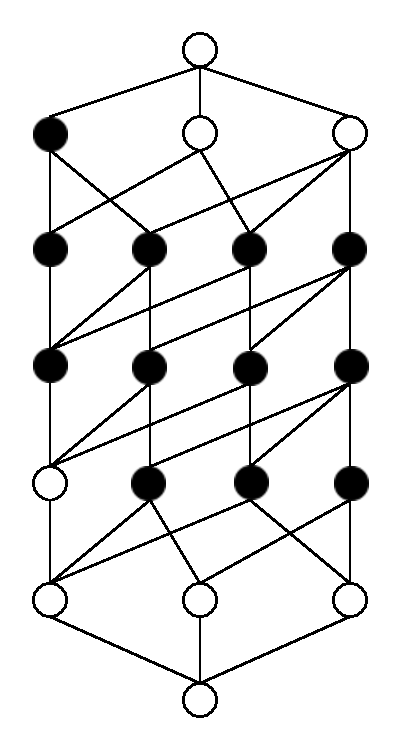
\includegraphics[scale=0.7]{counterexamplegraph.pdf}
\end{center}
%%%%%%%%%%%%%%%%%%%%%%%%%%%%%%%%%%%%%%%%%%%%%%%%%%%%%%%
\subsection*{Acknowledgements}
We thank Jonathan Novak (MIT) for guiding our research and providing helpful discussions.

%%%%%%%%%%%%%%%%%%%%%%%%%%%%%%%%%%%%%%%%%%%%%%%%%%%%%%%
% \bibliographystyle{plain} 
% \bibliography{myBibFile} 
% If you use BibTeX to create a bibliography
% then copy and past the contents of your .bbl file into your .tex file

\begin{thebibliography}{10}

\end{thebibliography}

\end{document}
